

%!TEX root = ../Notes.tex
\section{Homotopies} We now have enough background to start talking about geometric (or algebraic) topology. 
\begin{definition}
	Let $f$ be a path in $(X,F_X)$, and define $\overline{f} : I \to X$ by $\overline{f} (t) = f(1-t)$. 
\end{definition}

A few remarks: 
\begin{enumerate}
	\item $\overline{f}$ is a path, because it is a composition of continuous functions. 
	\item $\overline{f}$ is a path from $f(1)$ to $f(0)$. 
	\item $f \ast \overline{f} \neq $ the ``identity''. We haven't created an inverse. 
\end{enumerate}
\begin{definition}
	Let $(X,F_X)$ be a topological space, and $a\in X$. We define $e_a: I\to X$ by $e_a (t) = a$ for all $t\in I$. 
\end{definition}

However, note that $f\ast e_a \neq f$. This isn't an identity. 
\begin{definition}
	Let $(X,F_X)$ and $(Y,F_Y)$ be top spaces, and let $f_0: X \to Y$ and $f_1:X\to Y$ be continuous. Then we say that $f_0$ is \textbf{homotopic} to $f_1$ if there exists a function $F:X\times I \to Y$, continuous, such that $F(x,0) = f_0 (x)$, and $F(x,1) = f_1(x)$. We say that $F$ is a \textit{homotopy} from $f_0$ to $f_1$, and we write $f_0 \simeq f_1$. 
\end{definition}

This is probably the most important concept in the rest of these notes.

To illustrate homotopies, a couple of pictures.
\[ 

\includegraphics[width=300pt]{images/homotopy/circle_and_square} \]

It is visually apparent that one image can be warped to make the other, so $f_0$ and $f_1$ are homotopic. However, homotopic functions need not be homeomorphic. 

These are homotopic, for example:
\[ 

\includegraphics[width=300pt]{images/homotopy/circle_and_infty} \]
\begin{example}
	Let $X = I$ and $Y = \R^2$. Define $f_0: I \rightarrow \R^2$ by $f_0(x) = (x,0)$, $f_1: I \rightarrow \R^2$ by $f_1(x) = (x,x^2)$, and $F: I \times I \rightarrow \R^2$ by $F(x, t) = t(x, x^2) + (1-t)(x, 0)$.
	
	Observe that $F$ is continuous. Note also that $F(x,0) = (x, 0) = f_0(x)$ and $F(x,1) = (x, x^2) = f_1(x)$.
	
	Thus $F$ is a homotopy. 
\end{example}

\subsection{Drawing Homotopies}

How to draw a homotopy:
\[ 
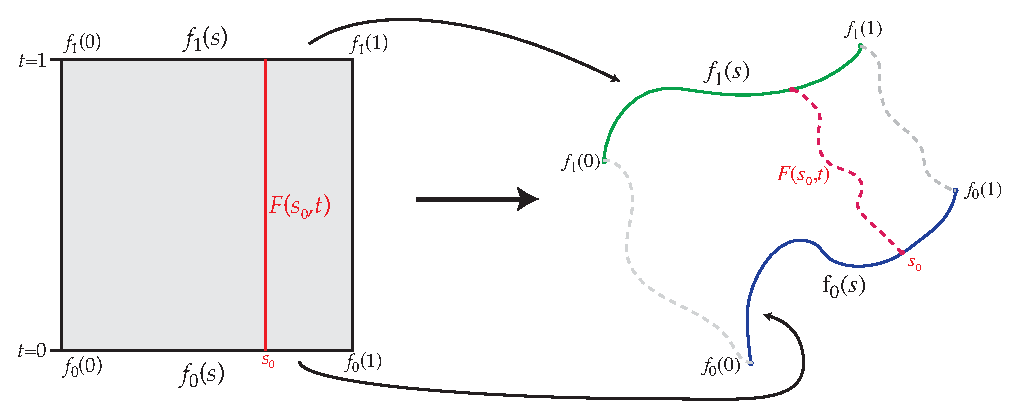
\includegraphics[width=350pt]{images/homotopy/how_to_homotope} \]

The image of a vertical segment in the square is the path taken by the $x$ coordinate of that segment during the homotopy.

A few remarks. 
\begin{enumerate}
	\item Suppose $Y$ is not path connected and $f_0(x)$ and $f_1(x)$ are in different path components. Then there does not exist a homotopy from $f_0$ to $f_1$.
	\[ 
	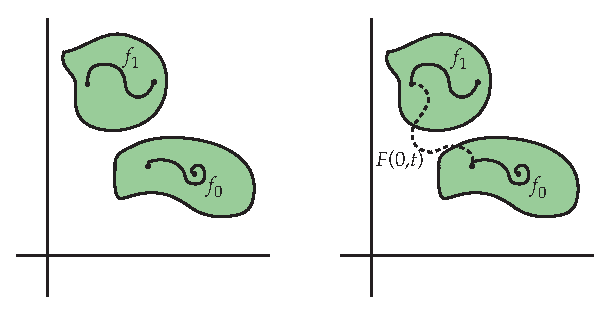
\includegraphics[width=300pt]{images/homotopy/not_path_connected} \]
	If $f_0$ and $f_1$ were homotopic, then $F(0,t)$ would be a path from $f_0(0)$ to $f_1(0)$. But $f_0$ and $f_1$ are in different path components.
	
	\item If $Y$ is path connected and $f_0$ and $f_1$ are paths in $Y$, then $f_0 \simeq f_1$. Homotope (the verb!) $f_0$ to its initial point, move it to the initial point of $f_1$ and then stretch it back out into $f_1$.)
	\[ 
	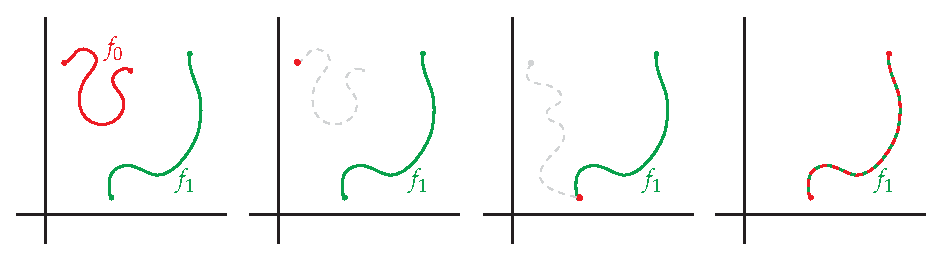
\includegraphics[width=450pt]{images/homotopy/paths_are_homotopic} \]
\end{enumerate}
\begin{example}
	Let $Y = \R^2 - \{(\frac{1}{2}, \frac{1}{3})\}$. Define $f_0: I \rightarrow Y$ by $f_0(s) = (s,s^2)$, and $f_1: I \rightarrow Y$ by $f_1(s) = (s,s).$ Because there's a hole in $Y$, we won't be able to just bend $f_0$ over to $f_1$.
	
	Define $G: I \times I \rightarrow Y$ by $G(s,t) = f_0((1-t)s)$. Observe that $G$ is continuous, and $G(s,0) = f_0(s)$ and $G(s,1) = f_0(0)$.
	
	Now define $H: I \times I \rightarrow Y$ by $H(s,t) = f_1(ts)$. Observe that $H$ is continuous and $H(s,0) = f_1(0)$ and $H(s,1) = f_1(s)$.
	
	Finally, define $F: I \times I \rightarrow Y$ by 
	\begin{displaymath}
		F(s, t) = \left\{ 
		\begin{array}{lr}
			G(s, 2t) & : t \in [0, \frac{1}{2}]\\
			H(s, 2t-1) & : t \in [\frac{1}{2}, 1] 
		\end{array}
		\right. . 
	\end{displaymath}
	\begin{itemize}
		\item[ $F$ is continuous: ] Let $A = I \times [0, \frac{1}{2}]$ and $B = I \times [\frac{1}{2}, 1]$. Both are closed in $I\times I$.\\
		$A \cap B = I \times \{\frac{1}{2}\}$. $G(s, 2(\frac{1}{2})) = G(s, 1) = f_0(0) = (0,0)$ and $H(s, 2(\frac{1}{2})-1) = H(s, 0) = f_1(0) = (0,0)$.
		
		Since $G$ and $H$ are continuous and agree at $A\cap B$, by the Pasting Lemma, $F$ is continuous.
		
		\item[$F$ is a homotopy : ]
		\[F(s, 0) = G(s, 0) = f_0(s) \qquad\text{and}\qquad F(s, 1) = H(s, 1) = f_1(s) \]
	\end{itemize}
	Thus $F$ is indeed an homotopy, and $f_0$ is homotopic to $f_1$! 
\end{example}

What path does $(1, 1)$ take during the aforementioned homotopy?

- Informally put, it moves down along $f_0$ and climbs back up $f_1$ to its old position.

More formally, 
\begin{displaymath}
	F(1, t) = 
	\begin{cases}
		G(1, 2t) & t \in [0, \frac{1}{2}]\\
		H(1, 2t-1) & t \in [\frac{1}{2}, 1] 
	\end{cases}
	= 
	\begin{cases}
		f_0(1-2t) & t \in [0, \frac{1}{2}]\\
		f_1(2t-1) & t \in [\frac{1}{2}, 1] 
	\end{cases}
	=\overline{ f_0} \ast f_1. 
\end{displaymath}

\subsection{Path Homotopies} 
\begin{definition}
	Let $f_0$ and $f_1$ be paths in $(X, F_X)$ from $a$ to $b$. We say $f_0$ is \textit{path-homotopic} if there exists a homotopy $F$ from $f_0$ to $f_1$ s.t. $\forall t \in I$, $F(0,t) = a$ and $F(1, t) = b$. We say $F$ is a \textbf{path homotopy} and write $f_0 \sim f_1$. 
\end{definition}
\[ 
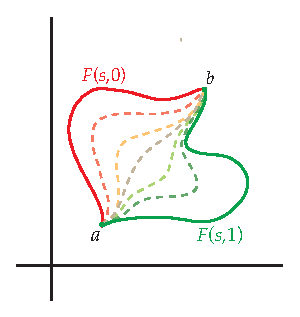
\includegraphics[width=200pt]{images/homotopy/path_homotopy} \]
\begin{example}
	Let $X$ be a convex region of $\R^n$, let $a$, $b \in X$, and let $f_0$ and $f_1$ be paths in $X$ from $a$ to $b$. 
\end{example}
Claim: $f_0 \sim f_1$. 
\begin{proof}
	Let $F(s,t) = (1-t)f_0(s) + tf_1(s)$ (Note: we call this the \textbf{straight line homotopy}). Observe that $\forall s \in I$, $F(s,0) = f_0(s)$ and $F(s,1) = f_1(s)$, and that $F$ is continuous, so $F$ is a homotopy from $f_0$ to $f_1$. Now let $t \in I$ be given. Observe that $F(0,t) = (1-t)f_0(0) + tf_1(0) = f_0(0) = a$, and that $F(1, t) = f_0(1) = b$. Thus $\forall t \in I$, $F(0,t) = a$ and $F(1,t) = b$, so $F$ is a path homotopy, and thus $f_0 \sim f_1$. 
\end{proof}
\begin{example}
	Let $X \cong D^2$, let $a, b \in X$, and let $f_0$ and $f_1$ be paths in $X$ from $a$ to $b$. Then $f_0 \sim f_1$. 
\end{example}
\begin{proof}
	Let $g: X \rightarrow D^2$ be a homeomorphism. Let $F: (I \times I) \rightarrow D^2$ be the straight line homotopy in $D^2$ from $g \circ f_0$ to $g \circ f_1$ (Note: $D^2$ is a convex region of $\R^2$, so by the last example we can use the straight line homotopy here).
	
	First, we need to show that $g^{-1} \circ F$ is continuous. Note that $F$ is continuous since $F$ is a homotopy. Note also that since $g$ is a homeomorphism, $g^{-1}$ is continuous. Thus $g^{-1} \circ F$ is the composition of continuous functions, and hence $g^{-1} \circ F$ is continuous.
	
	Now we need to show that $g^{-1} \circ F$ is a homotopy from $f_0$ to $f_1$.
	
	First, observe that $\forall s \in I$, $(g^{-1} \circ F)(s,0) = g^{-1}((1-0)g(f_0(s)) + (0)g(f_1(s))) = g^{-1}(g(f_0(s))) = f_0(s)$ since $g$ is a bijection, and similarly $(g^{-1} \circ F)(s, 1) = f_1(s)$. Thus, since $g^{-1} \circ F$ is continuous, $g^{-1} \circ F$ is a homotopy from $f_0$ to $f_1$.
	
	Lastly, we need to show that $g^{-1} \circ F$ is a \emph{path} homotopy.
	
	Note that $\forall t \in I$, $(g^{-1} \circ F)(0, t) = g^{-1}((1-t)g(f_0(0)) + tg(f_1(0))) = g^{-1}((1-t)g(a) + tg(a)) = g^{-1}(g(a)) = a$ since $g$ is a bijection. Similarly, $\forall t \in I$, $(g^{-1} \circ F)(1,t) = b$. Thus, since $g^{-1} \circ F$ is a homotopy from $f_0$ to $f_1$, $g^{-1} \circ F$ is a path homotopy, and thus $f_0 \sim f_1$. 
\end{proof}
\begin{theorem}
	Let $(X, F_X)$ be a topological space and let $a$, $b \in X$ be given. Then $\sim$ is an equivalence relation of paths in $X$ from $a$ to $b$. 
\end{theorem}
\begin{proof}
	In order to show $\sim$ is an equivalence relation, we need to show that $\sim$ is reflexive, symmetric, and transitive. 
	\begin{itemize}
		\item[Reflexive:] If $f$ is a path in $X$ from $a$ to $b$, let $F: (I \times I) \rightarrow X$ be given by $F(s,t) = f(s)$. Note that $F$ is a homotopy from $f$ to $f$ since, $\forall s \in I$, $F(s,0) = f(s)$ and $F(s,1) = f(s)$ and $F$ is continuous since $f$ is continuous. Observe that $\forall t \in I$, $F(0, t) = f(0) = a$ and $F(1, t) = f(1) = b$, so $F$ is a path homotopy and $f \sim f$. Thus, $\sim$ is reflexive. 
		\item[Symmetric:] Suppose that $f_1 \sim f_2$. Then there exists a path homotopy $F$ from $f_1$ to $f_2$ . Define $F': (I \times I) \rightarrow X$ given by $F'(s,t) = F(s, 1-t)$, $\forall (s,t) \in (I \times I)$. Note that $F'$ is continuous since $F$ is continuous so $F'$ is a composition of continuous functions. Recall that $F$ is a homotopy from $f_1$ to $f_2$, and thus $F'$ is a homotopy from $f_2$ to $f_1$ since, $\forall s \in I$, $F'(s, 0) = F(s, 1) = f_2(s)$ and $F'(s, 1) = F(s, 0) = f_1(s)$. Now observe that $\forall t \in I$, $F'(0,t) = F(0,1-t) = a$ and $F'(1,t) = F(1, 1-t) = b$, since $F$ is a path homotopy. Thus, $F'$ is a path homotopy, and thus $f_2 \sim f_1$, so $\sim$ is symmetric. 
		\item [Transitive:] Suppose that $f_1$, $f_2$, and $f_3$ are paths in $X$ from $a$ to $b$ s.t. $f_1 \sim f_2$ and $f_2 \sim f_3$. Since $f_1 \sim f_2$, there exists a path homotopy $F_1$ from $f_1$ to $f_2$, and since $f_2 \sim f_3$, there exists a path homotopy $F_2$ from $f_2$ to $f_3$. Define $F_3: (I \times I) \rightarrow X$ by 
		\begin{displaymath}
			F_3(s,t) = 
			\begin{cases}
				F_1(s,2t) & t \in [0, \frac{1}{2}]\\
				F_2(s,2t - 1) & t \in [\frac{1}{2}, 1] 
			\end{cases}
		\end{displaymath}
		
		Now we must show that $F_3$ is a path homotopy from $f_1$ to $f_3$. Observe that $A = I \times [0, \frac{1}{2}]$ and $B= I \times [\frac{1}{2}, 1]$ are closed in $I \times I$, and $F_1$ and $F_2$ are continuous, so if $F_1(s,t) = F_2(s,t)$ $\forall (s,t) \in A \cap B$, then by the pasting lemma $F_3$ is continuous. Since $A \cap B = I \times \{\frac{1}{2}\}$, and, $\forall s \in I$, $F_1(s, 2(\frac{1}{2})) = F_1(s, 1) = f_2(s)$ and $F_2(s, 2(\frac{1}{2}) - 1) = F_2(s, 0) = f_2(s)$, $F_3$ is continuous by the pasting lemma. Now, observe that $\forall s \in I$, $F_3(s, 0) = F_1(s, 2(0)) = F_1(s, 0) = f_1(s)$ and $F_3(s, 1) = F_2(s, 2(1) - 1) = F_2(s, 1) = f_3(s)$, so $F_3$ is a homotopy from $f_1$ to $f_3$. Now, observe that $\forall t \in I$, 
		\begin{align*}
			F_3(0,t) &= 
			\begin{cases}
				F_1(0,2t) & \mathrm{if }$ $ t \in [0, \frac{1}{2}]\\
				F_2(0,2t - 1) & \mathrm{if }$ $ t \in [\frac{1}{2}, 1] 
			\end{cases}
			\\
			&= 
			\begin{cases}
				a & t \in [0, \frac{1}{2}]\\
				a & t \in [\frac{1}{2}, 1] 
			\end{cases}
		\end{align*}
		(since $F_1$ and $F_2$ are path homotopies), and thus $F_3(0,t) = a$, $\forall t \in I$. Similarly, $\forall t \in I$, $F_3(1,t) = b$. Thus, $F_3$ is a path homotopy from $f_1$ to $f_3$, so $f_1 \sim f_3$, and thus $\sim$ is transitive. 
	\end{itemize}
	Thus, $\sim$ is an equivalence relation of paths in $X$ from $a$ to $b$. 
\end{proof}

Note that the same proof (using only the parts related to continuity and homotopy) works for $\simeq$. 
\begin{definition}
	Let $(X, F_X)$ be a topological space and let $a$, $b \in X$ be given. For each path $f$ from $a$ to $b$ in $X$, define $[f]$ to be the \textbf{path homotopy class of f}. 
\end{definition}
\begin{definition}
	Let $f$ be a path in $X$ from $a$ to $b$ and $g$ be a path in $X$ from $b$ to $c$. Define an \textsc{invisible symbol} by $[f][g] = [f \ast g]$. 
\end{definition}

Some remarks: 
\begin{enumerate}
	\item $[f]$, $[g]$, and $[f \ast g]$ are not elements of the same quotient `world' unless $a = b = c$. 
	\item We have to prove that invisible multiplication is well-defined, i.e. if $f \sim f'$ and $g \sim g'$, then we want $[f \ast g] = [f' \ast g']$ because $[f] = [f']$ and $[g] = [g']$. 
\end{enumerate}
\begin{lemma}
	[Important] The product of path homotopy classes is well-defined. Formally, let $(X,F_x)$ be a topological space. Let $f,f'$ be paths in $X$ from $a$ to $b$ and let $g,g'$ be paths in $X$ from $b$ to $c$. Then:
	\[f*g \sim f'*g' \Rightarrow [f][g] = [f'][g']\]
\end{lemma}
\begin{proof}
	We know $f*g$ and $f'*g'$ are paths in $X$ from $a$ to $c$ by a previous result. Let $F$ be the path homotopy from $f$ to $f'$, and let $G$ be the path homotopy from $g$ to $g'$.
	
	At this point, it may be wise to draw a homotopy diagram:
	\[ 
	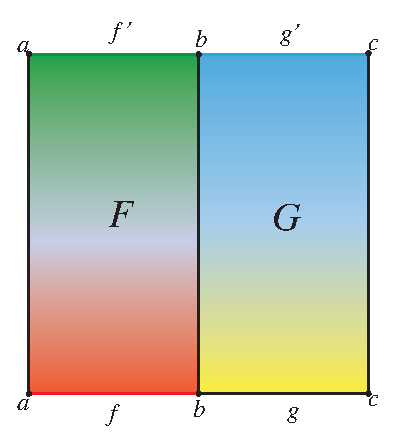
\includegraphics[width=150pt]{images/homotopy/product_well_defined} \]
	
	Define $H:I\times I\to X$ by:
	\[H(s,t) = 
	\begin{cases}
		F(2s,t) & s\in [0,1/2] \\
		G((2s-1),t) & s\in [1/2,1] 
	\end{cases}
	\]
	We claim $H$ is a homotopy from $f*g$ to $f'*g'$. We will now verify the claim. 
	
	We see that:
	\[F(2\cdot(1/2),t) = F(1,t) = b \qquad G(2\cdot(1/2) -1,t) = G(0,t) = b\]
	so by the pasting lemma, it follows that $H$ is continuous.
	
	We now show $H$ gives the desired paths by calculating:
	\[H(0,t) = F(0,t) = a \qquad H(1,t) = G(1,t) = c\]
	so $H(s,[0,1])$ gives a set of paths from $a$ to $c$. 
	
	Finally, we need to prove that $H$ gives a homotopy between the intended paths:
	\[H(s,0) = 
	\begin{cases}
		F(2s,0) & s\in [0,1/2] \\
		G(2s-1,0) & s\in [1/2,1] 
	\end{cases}
	= 
	\begin{cases}
		f(2s) & s\in [0,1/2] \\
		g(2s-1) & s\in [1/2,1] 
	\end{cases}
	= f*g \]
	Similarly:
	\[H(s,1) = 
	\begin{cases}
		F(2s,1) & s\in [0,1/2] \\
		G(2s-1,1) & s\in [1/2,1] 
	\end{cases}
	= 
	\begin{cases}
		f'(2s) & s\in [0,1/2] \\
		g'(2s-1) & s\in [1/2,1] 
	\end{cases}
	= f'*g' \]
	
	Consequently, $H$ satisfies the definition of a path homotopy from $f*g$ to $f'*g'$. We then have that $f*g\sim f'*g'$ so that by definition of the product of paths:
	\[[f][g] = [f*g] = [f'*g'] = [f'][g']\]
	as desired. 
\end{proof}
